% Created 2016-09-21 三 20:24
\documentclass[12pt]{ctexart}
\usepackage[utf8]{inputenc}
\usepackage[T1]{fontenc}
\usepackage{fixltx2e}
\usepackage{graphicx}
\usepackage{longtable}
\usepackage{float}
\usepackage{wrapfig}
\usepackage{rotating}
\usepackage[normalem]{ulem}
\usepackage{amsmath}
\usepackage{textcomp}
\usepackage{marvosym}
\usepackage{wasysym}
\usepackage{amssymb}
\usepackage[CJKbookmarks, colorlinks, linkcolor=black]{hyperref}
\tolerance=1000
\usepackage{wrapfig}
%\author{pal}
\title{胡月恒的简历}
\hypersetup{
  pdfkeywords={},
  pdfsubject={},
  pdfcreator={Emacs 25.1.1 (Org mode 8.2.10)}}
\begin{document}

\maketitle
\tableofcontents

\section{个人简历}
\label{sec-1}
\subsection{基本信息}
\label{sec-1-1}
%%%%%%%%%%%%%%%%%%%%%%%%%%%%%%%%%%%
\begin{wrapfigure}{r}{0.5\textwidth}
  \vspace{-25pt}
  \begin{center}
    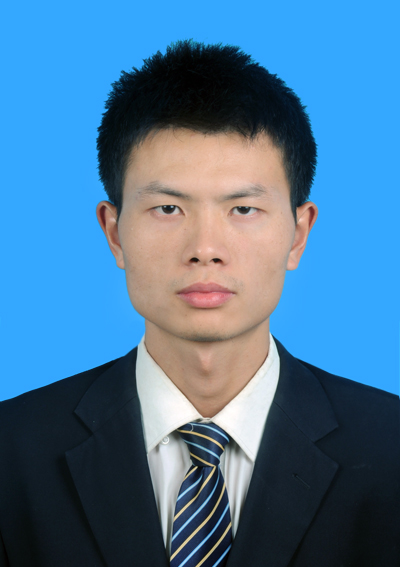
\includegraphics{portrait.jpg}
  \end{center}
\end{wrapfigure}
%%%%%%%%%%%%%%%%%%%%%%%%%%%%%%%%%%
\noindent{姓名:胡月恒\\}
性别:\ 男\\
应聘岗位:\ Java软件工程师\\
学历:\ 硕士(应届毕业生)\\
手机:\ 13323833820\\
邮箱:\ palagend@163.com\\
籍贯:\ 信阳\\
期望城市:\ 武汉+杭州+上海\\
出生年月:\ 1990\ -\ 10\ -\ 09\\
专业:\ 测试计量技术及仪器(嵌入式方向)\\
\subsection{技能描述}
\label{sec-1-2}
\subsubsection{Java}
\label{sec-1-2-1}
\begin{enumerate}
\item Java SE: Java语言基础, HTTP协议的握手与挥手机制, JVM的类加载机制, Java基本类库的使用;
\item Java EE: Servlet, JSP, JDBC, JPA;
\item 用过的框架:Spring, SpringMVC, Hibernate, MyBatis;
\item 熟悉的开发工具:Eclipse, Tomcat, Jboss, Atom;
\end{enumerate}
\subsubsection{Linux}
\label{sec-1-2-2}
\begin{enumerate}
\item Linux基础: Linux用户管理, Linux系统管理, Linux软件管理 ;
\item Linux服务器搭建: dhcp服务器搭建, apache服务器搭建, tftp服务配置, ssh服务配置;
\end{enumerate}
\subsubsection{数据库}
\label{sec-1-2-3}
\begin{enumerate}
\item 基础:SQL语言;
\item MySQL, Oracle;
\end{enumerate}
\subsubsection{其他}
\label{sec-1-2-4}
\begin{enumerate}
\item 客户端语言: Javascript;
\item 前段框架/库: jQuery, Angular, easyUI;
\item 服务端语言: Python, PHP, Node.js;
\item 终端设备: Android
\end{enumerate}
\subsection{教育经历}
\label{sec-1-3}
\noindent{2014年09月01日\ -\ 2017年06月01日 | 郑州大学 | 硕士研究生\\}
受教育类型: 全日制统分统招\\
研究方向: 嵌入式技术\\
院系: 物理工程学院\\
专业: 测试计量技术及仪器\\
主要专业课程: java程序设计,数值分析, 嵌入式技术,数字信号处理,光电探测技术,EDA技术\\
\\
2009年09月01日\ -\ 2013年06月01日 | 哈尔滨理工大学 | 本科\\
受教育类型:全日制统分统招\\
院系:测控技术与通信工程学院\\
专业:测试计量技术及仪器\\
主要专业课程: C/C++程序设计,MATLAB,测量方法,单片机编程,微机原理\\
\subsection{活动实践}
\label{sec-1-4}
\noindent{\textbf{校内活动}: 参见校羽毛球比赛|组织新同学聚会|参加院系迎新晚会的文艺演出;\\
\textbf{社会实践}: 参加由郑州大学委托给郑州达内科技组织的为期四个月的java软件实训活动.其间学习了JavaSE, JavaEE, Oracle, JavaScript等IT技术;练习项目主要有云笔记和电信运营商服务租赁计费系统.
\subsection{实习经验}
\label{sec-1-5}
\noindent{2016年03月07日\ -\ 2017年01月01日\\}
实习单位: 河南有线\\
职位:程序员\\
职位月薪(税前): 4000\\
工作描述: 本人在河南有线实习期间负责协助部门主管维护河南有线网络接入认证系统项目的维护和二次开发工作以及机房巡检工作.本人在工作中的主要贡献是: 1.对
旧代码做了部分优化,发现了程序读取配置信息的硬编码问题,将代码中的配置信息抽离到外部配置文件中,针对过于庞大的类进行分割,提高了程序的灵活性和健壮性. 2.
在机房巡检期间,利用实验服务器,自学并成功搭建了PXE安装linux操作系统的环境.\\
证明人:裴红星\ 导师\ 郑州大学\ 15690852281\\
\subsection{项目经验}
\label{sec-1-6}
\subsubsection{河南有线网络接入认证系统}
\label{sec-1-6-1}
\noindent{\textbf{项目描述}:这是我实习期间接受的第一个工作任务,为认证系统添加radius认证功能.这是一个比较老的项目,用的是EJB和jboss技术,框架采用的是struts.\\}
\textbf{项目经验}:第一次对旧项目做维护,感觉真的很棘手,因为之前并没有关注EJB和jboss,对struts这一过时的技术更是直接忽略;但是既然接手了任务,也只能
硬着头皮往前冲了.我先是花了一个晚上的时间恶补了EJB和jboss的知识,然后写了一些小demo练练手熟悉熟悉.等了解RMI的工作原理,jboss和tomcat之
间的关系之后,思路就清晰多了;接下来是阅读项目源码,理清逻辑结构(代码没有文档,真的很痛苦,花了不少时间).通过与业务人员的沟通,了解RADIUS认证的业务流程
,然后就是写代码了,根据OSS传过来的指令,对RADIUS数据库作相应的CRUD操作(小case).回过头来想想这整个过程,大多时间是用在学习消化新知识上面了
,而写代码本身并没有占用太多时间.这种经验,在课堂上肯定是学不来的.
\subsubsection{基于百度地图SDK的手机定位App}
\label{sec-1-6-2}
\noindent{\textbf{涉及的技术}:Baidu LBS,Android,java\\}
\textbf{开发工具和平台}:Android Studio,android手机\\
\textbf{项目描述}:这是我作毕业论文期间需要采集车辆行驶数据而编写的一个手机端定位数据采集App,功能比较简单,就是采集驾驶员行车时的定位数据并保存到本地文件中,供后期分析处理;\\
\textbf{项目收获}:本人主要学的是java,而安卓与java有着千丝万缕的亲缘关系,我也就尝试着做了一个android app.从android开发环境的搭建,到百度SDK的学习,从程序设计,在到app发布.整个过程都是自力更生,摸石头过河走过来的.虽然是半道出家搞android,但整个过程让我对android系统有了深入的了解.如果将来有转到android开发的需求应该不会太辛苦.\\
\subsubsection{博客发布系统}
\label{sec-1-6-3}
经过之前糟糕的开发体验,我也找了自身的原因,技能还是不扎实,面对快节奏时才会手忙脚乱.于是抽了一段时间学习Spring的源码,并结合设计模式的书籍理解大神的设计艺术,但是总有点空空的感觉;于是我想到做一个玩具项目当做自己的练兵场,尽量把平时学到的新知识运用到这个项目中以巩固自己.项目托管在Github上(\href{http://github.com/palagend/luna}{博客发布系统}),git的版本控制日志可以当做自己的学习笔记.
\subsection{所获奖项和证书}
\label{sec-1-7}
全国大学生电子设计大赛一等奖;
CET-6(440);
高级软件工程师;
高级数据库管理工程师;
系统分析师;
研究生学业奖学金;
优秀班干部;
驾驶证;
\subsection{兴趣爱好}
\label{sec-1-8}
捣鼓linux,看博客,读书,听歌,爱运动
\subsection{自我评价}
\label{sec-1-9}
\begin{enumerate}
\item 自学能力强. 当我面对陌生的新技术时,不会束手无策,而是通过上网搜索或是翻阅书籍自主学习新知识;在检索信息的过程中注重检索技巧, 首先粗略搜索,逛逛论坛看看博客,获取感性上的认识;然后,逐步缩小搜索范围,再阅读官方英文文档深入研究,直到get新技能.
\item 专注. 当我想做成一件事时,会自动屏蔽外界的干扰,整个脑子都被自己所想的事情给占据了,这样的发呆状态甚至会被朋友误以为抑郁了.
\item "悲观"的豁达者. "悲观"是指,不大相信生活会有什么奇迹发生,对任何事情都是做好最坏的打算,然后想出尽可能多的应对方案.豁达是指,对木已成舟的过往琐事不去懊悔计较,免得让自己心烦.大概就是"听天命,尽人事"的意思吧.
\end{enumerate}
% Emacs 25.1.1 (Org mode 8.2.10)
\end{document}